\documentclass{beamer}
\usepackage{ngerman}
\usepackage{graphicx}
\usetheme{Madrid}
\title{Algorithmen I Tutorium}
\author{Florian Tobias Schandinat}
\date{21.04.2011}
\institute{FTS}


\begin{document}


\begin{frame}
\frametitle{Willkommen}
\begin{block}{Algorithmen I Tutorium 19}
\begin{description}
\item[Wer?] Florian Tobias Schandinat\\
\item[Wo?] 50.34, Raum -118\\
\item[Wann?] jeden Donnerstag 15:45-17:15
\end{description}
\end{block}

\begin{block}{Material online}
http://github.com/schandinat/algorithmen1\_ss11
\end{block}
\end{frame}


\begin{frame}
\frametitle{Organisatorisches}
\begin{block}{"Ubungsbetrieb}
14 t"agig\\
Abgabe freiwillig, es gibt \alert{keinen} "Ubungsschein!\\
Abgabe aber gerne gesehen und zur Klausurvorbereitung hilfreich
\end{block}
\vspace{1cm}

\pause

\begin{center}
\textbf{\Huge Fragen?}
\end{center}
\end{frame}


\begin{frame}
\frametitle{Motivation}
\begin{alertblock}{Warum "uberhaupt mit Algorithmen besch"aftigen?}
Algorithmen spielen bei allt"aglichen Problemen eine wichtige Rolle
Algorithmen legen Eingenschaften von Programmen fest
Algorithmenanalyse ist auch in der Theorie wichtig
\end{alertblock}

\pause

\begin{block}{Wobei hilft es?}
\begin{itemize}
\item Wann wird mein Programm fertig? {\tiny in 2 Stunden oder 100 Jahren?}
\item Reicht der zur Verf"ugung stehende Speicher aus?
\item Welche Algorithmen/Datenstrukturen muss ich einsetzen um die Anforderungen zu erf"ullen?
\end{itemize}
\end{block}
\end{frame}


\begin{frame}
\frametitle{O-Kalk"ul}

\pause

\begin{block}{Asymptotisches Wachstum}
\pause
\begin{description}
\item[$f = o(g)$] $f$ w"achst asymptotisch langsamer als $g$
\item[$f = O(g)$] $f$ w"achst asymptotisch h"ochstens genau so schnell wie $g$
\item[$f = \theta(g)$] $f$ w"achst asymptotisch genau so schnell wie $g$
\item[$f = \Omega(g)$] $f$ w"achst asymptotisch mindestens genau so schnell wie $g$
\item[$f = \omega(g)$] $f$ w"achst asymptotisch schneller als $g$
\end{description}
\end{block}

\pause

\begin{block}{Hinweis}
$$f = \theta(g) \Longleftrightarrow f = O(g) \wedge f = \Omega(g)$$

\end{block}
\end{frame}


\begin{frame}
\frametitle{O-Kalk"ul in der Praxis (1)}
\begin{exampleblock}{}
for i = 1 to 5 $\cdot$ n\\
	\hspace{1cm} // tue etwas sinnvolles\\[0.5cm]
\pause
$\Longrightarrow O(n)$
\end{exampleblock}

\pause

\begin{exampleblock}{}
for i = 1 to n\\
	\hspace{1cm} // tue etwas sinnvolles\\
for i = 1 to n\\
	\hspace{1cm} // tue noch mehr sinnvolles\\[0.5cm]
\pause
$\Longrightarrow O(n)$
\end{exampleblock}
\end{frame}


\begin{frame}
\frametitle{O-Kalk"ul in der Praxis (2)}
\begin{exampleblock}{}
// tue etwas sinnvolles\\[0.5cm]
\pause
$\Longrightarrow O(1)$
\end{exampleblock}

\pause

\begin{exampleblock}{}
for i = 1 to n\\
	\hspace{1cm} for j = i to n\\
		\hspace{2cm} // tue etwas sinnvolles\\[0.5cm]
\pause
$\Longrightarrow O(n^2)$
\end{exampleblock}
\end{frame}


\begin{frame}
\frametitle{O-Kalk"ul in der Praxis (3)}
\begin{exampleblock}{Wie k"onnte ein nicht-polynomialer Algorithmus aussehen?}
Daten sind mit einem n-Bit Schl"ussel (zB $n = 256$) verschl"usselt worden. Finde den passenden Schl"ussel.\\[0.5cm]
Annahme: Es gibt keine Schwachstellen, nur Ausprobieren ist m"oglich!\\[0.5cm]
\pause
Dann gibt es $2^n$ m"ogliche Schl"ussel\\
$\Longrightarrow$ Algorithmus nicht polynomial zur Schl"ussell"ange
\end{exampleblock}
\end{frame}


\begin{frame}
\frametitle{O-Kalk"ul}
\begin{center}
\textbf{\Huge Fragen?}
\end{center}
\end{frame}


\begin{frame}
\frametitle{Sortieren}
\begin{block}{Sortieralgorithmen}
\begin{itemize}
\item Bubblesort
\item Insertionsort
\item Selectionsort
\item Mergesort
\item Quicksort
\item Radixsort
\end{itemize}
\end{block}
\end{frame}


\begin{frame}
\frametitle{Sortieralgorithmen -- "Ubung}
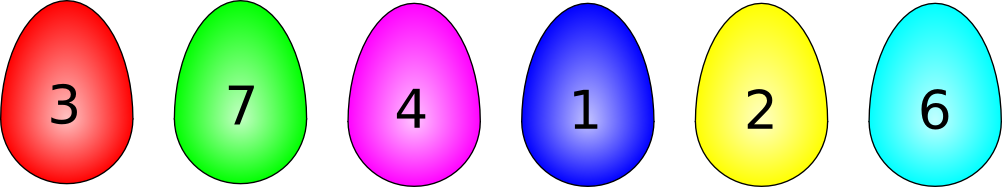
\includegraphics[scale=0.55]{eggs_unsorted}

\pause

\begin{exampleblock}{Sortieren sie die Eier in aufsteigender Reihenfolge mit}
\begin{itemize}
\item Bubblesort\pause
\item Insertionsort\pause
\item Selectionsort\pause
\item Mergesort\pause
\item Quicksort\pause
\item Radixsort
\end{itemize}
\end{exampleblock}
\end{frame}


\begin{frame}
\frametitle{Sortieralgorithmen}
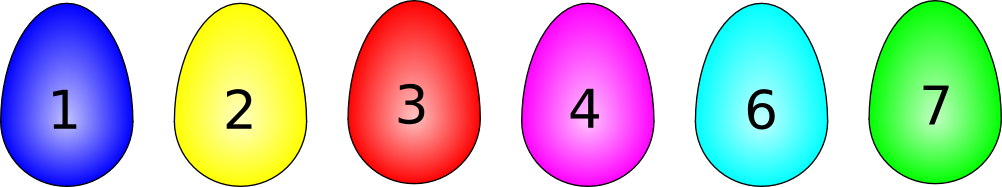
\includegraphics[scale=0.55]{eggs_sorted}
\vspace{1cm}

\begin{center}
\textbf{\Huge Fragen?}
\end{center}
\end{frame}


\begin{frame}
\frametitle{1. "Ubungsblatt}

\pause

\begin{center}
\textbf{\Huge Weitere Fragen? (Pseudocode, Suchen, ...)}
\end{center}
\end{frame}


\begin{frame}
\frametitle{Ende}
\begin{center}
\textbf{\Huge Vielen Dank f"ur die Aufmerksamkeit}
\end{center}


\begin{center}
\textbf{\Huge und sch"one Osterfeiertage!}
\end{center}
\end{frame}


\end{document}
